\documentclass[a4paper, 12pt]{article}
\usepackage[utf8]{inputenc}
\usepackage[T1]{fontenc}
\usepackage[scale=.8]{geometry}
\usepackage[french, english]{babel}
\usepackage{hyperref}
\usepackage{graphicx}
\usepackage{amsmath}
\usepackage{amssymb}
\usepackage{setspace}

\title{\textbf{Sécurité des données dans le cloud}\\~\\Que représente la
sécurité informatique dans le domaine du cloud ?}
\author{}
\date{}

\begin{document}
  \begin{spacing}{1.1}
  \renewcommand{\thepage}{}

  \maketitle
  \rule{\linewidth}{0.4mm}

  \vspace*{2.6cm}
  \begin{center}
    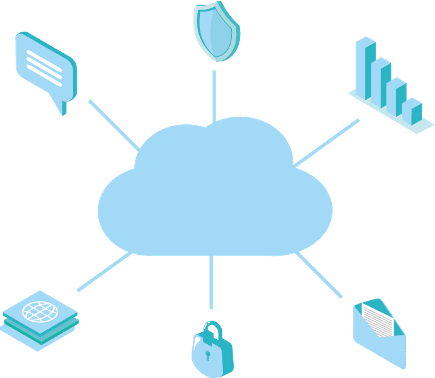
\includegraphics[scale=.5]{img/cloud.png}
  \end{center}

  \vspace*{4.4cm}
  \begin{minipage}{.6\linewidth}
    Enzo CADONI - Jean CHAPUT - Evan SEDENO
  \end{minipage}
  \begin{minipage}{.4\linewidth}
    
\includegraphics[scale=.34]{./img/logo.png}
  \end{minipage}

  \newpage
  \tableofcontents
  \newpage

  \renewcommand{\thepage}{\arabic{page}}
  \setcounter{page}{1}
  \selectlanguage{french}
  \begin{abstract}
    Ce rapport présente une étude sur ce que peut représenter la sécurité
    informatique dans le domaine du cloud. Nous distinguerons d'abord quels
    peuvent être les phénomènes et les failles pouvant mener à des perte ou à
    des vols de données sur le cloud. Ensuite, nous exposerons des techniques
    actuelles permettant de se prémunir avec plus ou moins d'efficacité de ces
    failles. Enfin, nous nous demanderons si dans l'avenir, l'intelligence
    artificielle ne pourrait pas être une solution particulièrement viable dans
    l'anticipation des risques et des menaces concernant le cloud.
  \end{abstract}

  \selectlanguage{english}
  \begin{abstract}
    This study report deals with the security in the cloud computing domain and
    what it can represent. We will first discuss about how a cloud can be
    exposed to security breaches, and what they are. Then, we will expose some
    of the current techniques that can, with more or less efficacity, protect
    the cloud from those breaches. To conclude, we will ask ourselves if the
    artificial intelligence could be an efficient way to prevent cloud breaches
    and attacks in the future.
  \end{abstract}

  \newpage
  \selectlanguage{french}
  \section{Introduction}
    Aujourd'hui, une majorité de nos données personnelles, professionnelles,
    publiques comme privées, transitent par des services de stockage en ligne,
    des données qui peuvent aller de simples images publiques à des données
    confidentielles pouvant mettre en péril des entreprises, des collectivités
    ou même des nations. \\

    Le cloud désigne l'ensemble des serveurs auquel on peut accéder en ligne,
    ces serveurs peuvent héberger non seulement des données, mais aussi des
    services, des logiciels, etc. Des entreprises comme Microsoft, Amazon ou
    encore OVHCloud proposent de louer des serveurs afin que les particuliers
    comme les entreprises puissent héberger des services en ligne. On distingue
    ici quatre modèles de cloud proposé par les fournisseurs, le modèle sur
    site, IaaS, PaaS et SaaS, \footnote{aaS signifie as-a-Service, cette mention
    signifie qu'un fournisseur prend en charge la gestion du service et de
    certaines fonctionnalités pour les utilisateurs}. Les trois modèles
    diffèrent dans le nombre d'aspects du cloud qui est géré par le fournisseur
    et non par le client. On peut voir dans l'annexe \ref{fig:modeles} ce qui
    différencie les différents modèles proposés. \\

    Un bon moyen de visualiser l'ampleur que le cloud a pris dans le monde est
    de l'illustrer par quelques statistiques

    \begin{itemize}
      \item Environ 94\% des entreprises utilisent des services de cloud.
      \item En 2025, selon les prévisions actuelles, 100 zettabytes de données
            devraient être stockées sur des services en ligne
            \footnote{Cela représente 10$^{23}$ octets de données soit
            10$^{11}$ disques durs de 1To}.
      \item En 2013, au total, seulement un exabyte de données était stocké
            sur des services de cloud\footnote{100 zettabytes = 100000
            exabytes}.
    \end{itemize}

    On peut voir par ces quelques statistiques que non seulement le nombre de
    données stockées en ligne est gigantesque, mais aussi qu'il croit très
    rapidement, il est donc nécessaire de se prémunir contre les risques
    potentiellement encourus. \\

    Afin de visualiser ce que représente la sécurité dans le cloud, il va être
    nécessaire de se demander ce qui peut le menacer, quel genre de faille
    pourrait menacer un tel service, sont elles seulement techniques ?. Ensuite,
    il sera pertinent d'observer les façons d'anticiper les menaces, et quelles
    sont les protocoles déjà établis pour s'en prémunir. Enfin, on pourrait se
    demander ce qu'il manque aujourd'hui dans le domaine de la sécurité des
    services cloud, et si l'intelligence artificielle ne pourrait pas nous aider
    à détecter des attaques en cours ainsi qu'à prévenir les failles de
    sécurité.

  \section{Les risques menaçant l'intégrité des données}
    L'inquiétude suscitée par le cloud est que ce genre de service héberge
    souvent beaucoup d'utilisateurs. Si un attaquant réussit à pénétrer un
    cloud, il met la main sur les données de l'intégralité des personnes qui en
    font l'usage. Nous allons donc voir ce qui pourrait permettre à un attaquant
    de pouvoir voler les données stockées en ligne dans ce type de service.

    \subsection{Différentes erreurs humaines}
      La grande majorité des failles qui ont mené à des vols ou pertes de
      données sur un cloud proviennent, comme pour une grosse partie des
      systèmes informatiques actuels, d'une erreur humaine. Une mauvaise
      application d'une routine\footnote{Les anglophones parlent de workflow}
      lors d'un changement de configuration ou d'architecture peut mener
      l'ouverture d'une brèche.

      \subsubsection{Défauts de configuration}
        La configuration d'un service cloud est essentielle, c'est elle qui va
        permettre d'assigner des droits aux utilisateurs et c'est par elle que
        l'on va pouvoir mettre en place les mesures de sécurité du service si le
        fournisseur de solutions ne prend pas en charge cette tâche. Des
        configurations de ce genre de service peuvent être source d'erreurs et
        mener à l'ouverture de failles. On sait que c'est le modèle
        \textbf{IaaS} qui est mis en cause dans la plupart des cas. En effet, ce
        modèle de cloud est très flexible et permet aux utilisateurs/entreprises
        de pouvoir configurer et gérer de nombreux aspects du cloud qu'ils
        utilisent, en les configurant potentiellement d'une façon trop peu
        sécurisée. Pour citer l'étude [AF2019], "\textit{about 99\% of
        misconfigurations go unnoticed by companies using IaaS}".
        \footnote{Traduction : Environ 99\% des erreurs de configurations ne
        sont pas remarquées par les entreprises utilisant le modèle IaaS}.

      \subsubsection{Mauvaise gestion du contrôle d'accès}
        Un cas particulier très répandu quand on parle de mauvaise configuration
        est une mauvaise gestion du contrôle d'accès des utilisateurs du
        service. Parfois, un trop grand nombre de personnes l'utilisant peuvent
        avoir accès à des données sensibles, par exemple au sein d'une
        entreprise, sans pour autant que cela soit nécessaire. Ce phénomène
        découle d'un manque de contrôle de ces accès. Laisser à trop de
        personnes l'accès à des données sensibles multiplie le risque d'attaque.
        On peut imaginer un attaquant extérieur qui pourrait vouloir pénétrer le
        stockage par ricochet en utilisant les utilisateurs concernés, mais
        aussi les utilisateurs eux-mêmes qui pourraient cacher un attaquant
        interne, il est donc nécessaire d'assurer un contrôle des accès
        rigoureux.

        On peut ici citer l'exemple de la plateforme Twitch\footnote{
        \url{Twitch.tv} est une plateforme permettant de diffuser du contenu en
        direct sur internet.}. En effet, après un mauvais changement de
        configuration du serveur, beaucoup trop de personnes travaillant dans
        l'entreprise on pu avoir accès au code source et à certaines données
        sensibles. Ces salariés ne n'étaient pas accrédités à voir ce contenu
        avant cet événement, certains ont pu en profiter pour voler des données
        de l'entreprise. La plateforme aurait perdu, à cause de ce défaut de
        configuration, 125Go de données, contenant des informations privées
        essentielles.

      \subsubsection{Sauvegardes et mots de passe}
        Lorsqu'on parle d'un service géré par exemple par une entreprise, il est
        nécessaire de parler de sauvegardes. En effet, pour s'assurer de perdre
        le moins de données en cas de suppression accidentelle, ou bien
        volontaire par un éventuel attaquant. Ce qui peut-être très courant est
        bien sur une sauvegarde d'une ou plusieurs base de données. Une erreur
        pourrait de ne pas faire attention où l'on stocke cette sauvegarde.
        Contenant des données sensibles comme par exemple des mots de passe,
        il est important de faire attention à l'endroit prévu pour stocker de
        telles sauvegardes.

    \subsection{La gestion de la mémoire dans le cloud}
      À l'image d'un disque dur de taille normale, le cloud est un espace de
      stockage partagé par plusieurs systèmes et/ou utilisateurs, il est
      important de se concentrer sur la gestion de l'espace alloué à chacun. \\

      Un des problèmes cité page 3/4 de cette étude [VR2016] est le fait que la
      mémoire effacée peut être récupérée. En effet, \textit{"The resource
      allocated to a particular user may be assigned to the other user at some
      later point of time"}\footnote{Traduction : l'espace alloué à un
      utilisateur peut être assigné à un autre moment}. Les services de cloud
      marchent nécessairement avec un système d'allocation de mémoire dynamique
      en fonction de la requête d'espace de l'utilisateur. Les services n'ayant
      pas une quantité infinie de stockage, Un morceau de l'espace va surement
      être utilisé successivement par plusieurs utilisateurs différents.
      L'utilisateur de ce morceau de l'espace pourra donc potentiellement
      récupérer d'anciennes données effacées qui ne lui appartiennent pas.

      En effet, sur la plupart des machines, il est possible de récupérer des
      données qui ont été effacés, les données ne sont en réalité pas réellement
      effacées. Lorsqu'on supprime un fichier sur un système, par exemple un
      système \verb+UNIX+ avec la commande \verb+rm+, ce dernier supprime la
      référence vers le fichier, pas son contenu. Celui-ci est donc toujours
      disponible si l'on possède une autre référence y menant, et de manière
      générale, n'est pas supprimé tant que le disque ou le dispositif de
      stockage n'a pas réécrit d'autres données par-dessus. Si un utilisateur
      dispose d'un morceau de la plage mémoire allouée précédemment à un autre
      utilisateur, il pourra donc tenter de les récupérer.

      \begin{figure}[h]
        \centering
        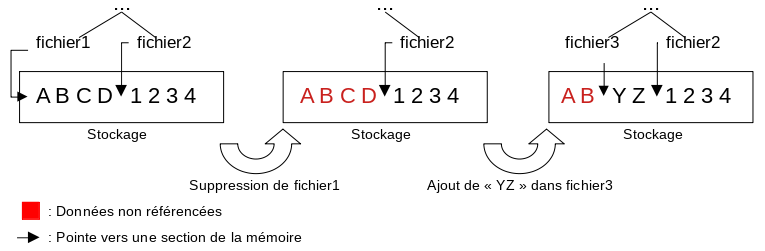
\includegraphics[scale=.6]{img/schema_memoire.png}
        \caption{Illustration du comportement du stockage durant une suppression
        basique}
      \end{figure}

      Un autre problème posé par le partage massif du cloud est la fragmentation
      de la mémoire. En effet, un problème pourraient résider dans la mauvaise
      ségmentation de celle-ci. Ceci pourrait permettre l'accès au même
      morceau de mémoire par plusieurs personnes, et un utilisateur pourrait
      voler des données à un autre, ou même récupérer des données supprimées
      comme dit plus haut.

    \subsection{Risques physiques}
      Les clouds sont des espaces de stockages, il est aussi nécessaire de
      considérer les menaces liées aux supports de stockages physiques des
      données comme les centres de stockages. On sait que la perte de données
      à proprement parler est peu probable quand on applique le principe de
      \textbf{redondance}. Ce principe repose dans le fait de posséder plusieurs
      sauvegardes du système et des données à plusieurs endroits
      géographiquement différents. La probabilité pour qu'une intempérie ou un
      problème matériel touche tous les centres de données utilisés est donc
      diminuée. La redondance permet donc de se prémunir des problèmes de ce
      type, mais pas des vols de données. \\

      Néanmoins, un centre de données peut bel et bien être victime de
      sinistres, causant la perte de nombreuses données. On peut penser à
      l'incendie qui avait frappé le centre de données d'OVHCloud à Strasbourg.
      De nombreux utilisateurs, particuliers comme des entreprises, ont perdu de
      nombreuses données. Même des services gouvernementaux et des médias furent
      impactés par l'incident.

      Il est aussi nécessaire de réfléchir à la protection humaine des centres
      de données. On peut imaginer des attaquants essayer de pirater
      physiquement un centre de données.

  \section{Anticipation et prévention des risques}
      L'identification des risques liés à une installation dans le cloud est
      primordiale car elle permet de pouvoir réfléchir à des solutions pour
      anticiper les attaques et les solutionner. Puisqu'il existe de nombreux
      risques dont une partie ont été traités dans la partie précédente, il
      existe un grand nombre de méthodes et de solutions pour les anticiper
      et les éviter.

      \subsection{Un aspect social}
      Le domaine de l'ingénierie sociale est en hausse car il s'agit très
      certainement de la méthode la plus simple et non la moins efficace pour
      obtenir l'accès à des données ou des services illégitimement. Il est
      crucial pour quiconque s'intéresse à la technologie du cloud et d'autant
      plus pour les entreprises de se former et de former l'ensemble des
      équipes, par exemple au sein, d'une entreprise, aux risques bien réels
      auxquels ils peuvent faire face dans leur quotidien. \\

      Pour une entreprise fournissant des services cloud, il est aussi
      nécessaire de définir clairement des règles de conduite pour l'ensemble du
      personnel afin d'éviter au maximum les failles de sécurité sensibles à
      l'ingénierie sociale. D'autant plus que ce sont des failles critiques qui
      peuvent parfois mener à des pertes conséquentes sur l'ensemble des données
      hébergées. \\

      Pour revenir sur un court exemple, on pourrait citer l'attaque subie par
      l'entreprise Uber en 2022 qui a eu lieu suite à un fait d'ingénierie
      sociale qui a permis à un attaquant l'accès à l'un des comptes
      administrateur de l'entreprise. Avec une politique de conduite plus
      stricte et une mise en garde sur les risques, l'attaque aurait pu être
      détectée plus tôt, ou même évitée. \\

    \subsection{Sur le plan physique}
      Les clouds étant des espaces de stockages numériques auxquels un
      utilisateur a très peu voire pas du tout d'accès sur le plan physique.
      Qu'il soit un particulier ou une entreprise, lorsqu'un utilisateur
      prévoit de souscrire à un service cloud, il devient alors nécessaire de
      procéder à une étude des risques physiques liés au fournisseur de
      ce service et à la politique de sécurité qu'il applique au sein de ses
      infrastructures. Y a-t-il de la surveillance, des contrôles d'accès ou
      d'autres mesures permettant de garantir un accès limité au site ? Il
      existe notamment certaines certifications qui peuvent être utilisées dans
      ce but comme la certification ISO 9000 \footnote{Certification délivrée
      par l'organisme ISO selon un certain nombre de critères comme
      l'organisation, les clients, les données, les systèmes etc.} ou SAS 70
      \footnote{State on Auditing Standards no. 70, remplacée par SSAE16. Il
      s'agit d'une certification spécialisée pour les centres de données} par
      exemple. De plus, certains fournisseurs de cloud ont une politique de
      confidentialité concernant l'emplacement et les spécificités de leurs
      datacenters afin de se prémunir contre les menaces. \\

      Tout cela étant dit, une perte de données ou une rupture d'accès à un
      service dans le cloud ne provient pas toujours d'une action volontaire
      d'un ou plusieurs individus. C'est pour cela que le contrôle d'accès et la
      surveillance ne suffisent pas à garantir la sécurité des données ou
      du service. Il est aussi nécessaire de se prémunir des risques liés à des
      catastrophes naturelles comme les incendies, les inondations ou bien plus
      simplement des coupures de courant par exemple. Cela peut-être
      effectué en prévoyant une redondance des données grâce à des sauvegardes
      régulières chiffrées et stockées dans d'autres infrastructures.

      Dans le cadre d'un service qui outrepasserait le simple stockage de
      données, il est aussi nécessaire de prévoir une redirection du service
      vers une autre plateforme fonctionnelle. Cela permet d'éviter les
      interruptions de service pour des applications cloud qui y seraient
      sensibles.

    \subsection{Sur le plan technique}
      L'une des difficultés d'un système dans le cloud réside dans les
      responsabilités d'actions ambiguës. En effet, si l'on considère les
      trois types de cloud, à savoir IaaS, PaaS et SaaS, il est parfois
      difficile pour un utilisateur de comprendre quelles actions sont à
      sa charge et quelles actions sont prises en charge par le fournisseur. \\

      Dans le cas d'un cloud SaaS, l'utilisateur a très peu de contrôle sur
      la manière dont les choses vont fonctionner à l'intérieur de sa machine.
      En réalité, l'ensemble de la configuration système et logicielle sur
      laquelle va reposer son service est aux mains du fournisseur d'accès.
      Cela a de nombreux avantages puisque l'ensemble des coûts d'architecture
      et de sécurisation sont finalement gérés par le fournisseur de services
      qui garantit en plus de cela un niveau de sécurité en théorie plus
      intéressant du fait de son expertise sur ses propres systèmes. Un point
      crucial et pourtant évident reste cependant aux mains de l'utilisateur.
      Il s'agit du choix de moyens d'authentification aussi sécurisés que
      possible, quitte à utiliser de l'authentification multifactorielle voir
      de l'expiration de mots de passe. Il s'agit là du seul point vraiment
      sensible de cette configuration. \\

      L'utilisation d'un cloud de type PaaS n'est pas très différente de
      celle d'un SaaS d'un point de vue sécurité informatique. L'utilisateur
      n'aura pas non plus à s'occuper de la configuration système et logicielle
      qui reste ainsi au fournisseur. Cependant un utilisateur de ce type de
      cloud devra se charger de la sécurité des applications qu'il décidera de
      déployer sur le système ainsi que de leurs services associés comme les
      bases de données par exemple. La gestion de la sécurité de ces
      applications peut être déléguée à des experts, ou dans le cas d'une
      entreprise suffisamment importante, elle sera très certainement gérée
      par l'un des services de l'entreprise en question. \\

      Même si l'utilisation d'un cloud SaaS ou Paas semble idéale d'un point
      de vue sécurité pour la plupart des utilisateurs, il ne s'agit cependant
      pas d'une solution universelle puisque certains utilisateurs particuliers
      ou entreprises ont besoin de plus de flexibilité. Plus de flexibilité
      implique inévitablement plus de responsabilités. Ainsi sur un cloud de
      type IaaS, l'utilisateur se trouve pratiquement sur une machine vide sur
      laquelle il va devoir installer un système d'exploitation et procéder à
      sa configuration. Par-dessus ce système, il faut ensuite installer les
      logiciels et applications nécessaires. À ce moment là, sécuriser le
      système se rapproche finalement de ce que l'on connaissait par le passé
      quand chaque entreprise disposait de sa propre installation physique. \\

      La complexité de la sécurisation d'un système cloud réside plus souvent
      du côté du fournisseur de cloud tel qu'Azure, AWS, OVH et beaucoup
      d'autres. De ce côté-là chaque fournisseur développe ses propres
      technologies de sécurité. Les technologies et outils sont nombreux mais
      on peut citer les systèmes d'authentification basés sur les privilèges,
      les systèmes de monitoring et d'analyse du système ou bien des logiciels
      de chiffrement des données par exemple. \\

      Malgré les solutions qui existent aujourd'hui, la sécurité du cloud
      reste un des enjeux de ces prochaines années car il est encore difficile
      d'assurer une installation fiable de manière pérenne sans déployer de
      gros moyens financiers et humains.

  \section{L'avenir de la sécurité dans le cloud avec l'IA ?}
    Depuis la crise sanitaire causée par le COVID-19 en 2020, les organisations
    accélèrent leurs transformations numériques, en trouvant de nouvelles façons
    de travailler et de communiquer. La sécurité des organisations évolue petit
    à petit chaque jour, et les cybercriminels adaptent également leur façon
    d'attaquer les systèmes. Avec l’émergence de l'intelligence artificielle
    dans la cybersécurité, le système immunitaire des organisations peut
    fonctionner de manière autonome et s'adapter aux conditions inconnues et
    imprévisibles de chaque système et attaque.

    \subsection{La prévention par l'IA}
      Avec les bonnes données, l'apprentissage machine peut permettre de prédire
      avec précision les événements futurs. Pour que cela fonctionne, les
      experts doivent recueillir beaucoup d'informations et les utiliser pour
      créer des modèles prédictifs. Ces données montrent donc comment divers
      événements pourraient se dérouler. En cybersécurité, les organisations
      peuvent comprendre les menaces potentielles et prédire ce qui pourrait
      arriver grâce à l'apprentissage machine. \\

      Pour l’instant, ces systèmes ne sont pas encore assez développés.
      Néanmoins, les perspectives de développement de l’IA\footnote{Intelligence
      Artificielle (AI en anglais)} préventive en cybersécurité se décomposent
      en deux types. Le premier type d'IA a besoin d’une grosse banque
      d'informations concernant les différentes attaques contre les
      organisations similaires qui ont déjà eu lieu. L'IA peut alors effectuer
      une évaluation précise des risques pour une entreprise donnée. Le deuxième
      type d’IA est beaucoup plus complexe, car celle-ci se repose sur le
      travail d’un White-Hat\footnote{Pirate éthique expert en cybersécurité qui
      réalise des tests d'intrusion et d'autres méthodes de test afin d'assurer
      la sécurité des systèmes d'information d'une organisation} en utilisant
      les ressources et reproduisant les attaques. Le principe ici est
      d’automatiser les tests d’intrusions réalisées par ces White-Hat afin de
      déceler les failles présentes dans un cloud.

    \subsection{La protection par l'IA}
      Les modèles actuels d'IA peuvent lutter en permanence contre les
      menaces. Beaucoup d’entreprises s'appuient sur ces outils pour la sécurité
      dans le cloud afin de prendre des mesures sans interruption. Une des idées
      communes sur systèmes d'IA est qu'ils peuvent répondre intelligemment aux
      attaques et ça instantanément. Cependant, il s'agit d'une idée fausse pour
      deux raisons principales. La première est que ces systèmes font uniquement
      des suggestions aux administrateurs, mais eux seul peuvent prendre des
      mesures lors d'une attaque. Ainsi, ces technologies ne font que suivre des
      règles simples et préalablement programmées. Ensuite, même si l’IA dans le
      cloud peut agir directement sur les systèmes, il existe toujours des
      limites. Bien cette technologie puisse empêcher certains utilisateurs
      d'accéder à certaines zones, les privilèges donnés sont généralement
      limités pour éviter toute mauvaise décision. \\

      L’intégration de l’IA dans un cloud pour la cybersécurité affecterait
      directement les systèmes de l’organisation ce qui comporte des risques
      importants. Si le système d'IA vient à prendre de mauvaises décisions, il
      pourrait éventuellement bloquer les utilisateurs et les systèmes, ce qui
      impacterait fortement les organisations.

    \subsection{Comment ça marche ?}
      Avant de prendre des mesures défensives, l’IA doit analyser le
      comportement de l’attaquant en réalisant une analyse préventive. Le
      système doit étudier premièrement les projections d’attaque, c’est-à-dire,
      est-ce qu’il va y avoir potentiellement un attaquant. Ensuite, il faut
      reconnaitre les intentions de celui-ci en trouvant son but grâce à des
      motifs déjà connus. Enfin, l’IA doit reconnaître le type d’attaque, quand
      et comment elle va se passer et les mesures qu’elle doit mettre en œuvre
      pour éviter ces attaques. Cette prévention, passant par la perception, la
      compréhension et la projection de ses attaques utilisent 3 types
      d’approches. Certaines méthodes se basent sur les mathématiques discrètes,
      d'autres sur un modèle mathématique continu, d'autres encore s'appuyant
      sur des techniques d'apprentissage machine et de fouille de données. Cette
      classification se base sur celle de l'étude [MJEP18]. \\


      On retrouve par exemple dans une de ces approches l’utilisation de graphes
      orientés pondérés pour prédire avec une certaine probabilité le prochain
      type d’attaque en fonction de la précédente. On peut voir dans la figure
      \ref{fig:1} un réseau bayésien\footnote{Aussi appelé graphe d'attaque
      bayésien.}. Les probabilités de ce réseau bayésien peuvent être calculées
      grâce à de l'apprentissage machine couplé à l'exploration des données de
      précédentes attaques. On peut aussi obtenir des données fiables d'un
      expert dans le domaine.

      Dans le graphe présenté en figure \ref{fig:1}, on peut distinguer dans le
      noeud \textit{D} l'attaquant. On sait qu'il attaque à distance et qu'il va
      utiliser une faille de dépassement de tampon, la probabilité qu'il essaye
      sur le serveur FTP est la plus élevée.

      \begin{figure}[h]
        \centering
        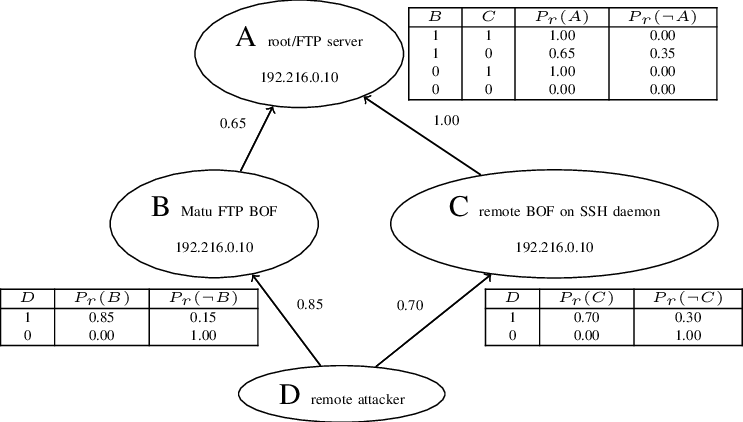
\includegraphics[scale=.5]{img/attackgraph.png}
        \caption{Graphe bayésien pondéré représentant une attaque potentielle.
        Source : [MJEP18]}
        \label{fig:1}
      \end{figure}

      L’IA s’assure plusieurs fois qu’il s’agit vraiment d’une attaque
      malveillante menaçant l’intégrité de l’entreprise. Une fois la menace et
      le type d’attaque identifié, il ne reste plus qu’à prendre des mesures
      contre cette attaque. L’IA sera limité aux accès que l’administrateur lui
      aura attribué. Celle-ci pourrait par exemple pouvoir bloquer la connexion
      aux serveurs pour une certaine adresse IP ou encore une certaine machine
      interne probablement infectée.

    \subsection{Solution viable ou non ?}
      Malgré de nombreuses idées fausses sur ce que l'IA peut réellement
      faire pour améliorer les systèmes de sécurité, cet outil joue un rôle
      important dans l'amélioration de la sécurité du cloud. Il a également de
      grandes perspectives d’évolution. L’IA pourrait contribuer à la pénurie de
      compétences en cybersécurité qui donne l'opportunité aux pirates de mener
      des activités illicites. Alors que cette technologie stimule déjà
      l'innovation et la protection contre les menaces, l'IA pourrait réduire
      les efforts des professionnels en cybersécurité et automatiserait le
      processus de protection. Alors que les pirates continuent d'améliorer
      leurs attaques, la mise en œuvre de l'IA dans la sécurité du cloud
      deviendra plus efficace. Toutes les cyber-opérations peuvent être
      entièrement automatisées avec une intervention humaine minimale. \\

      Actuellement, le problème de l’IA pour la cybersécurité dans le cloud est
      que les organisations l’utilisant se reposent trop sur elle, croyant que
      le système pourrait détecter et arrêter toutes les attaques. Comme dit
      précédemment, ces systèmes sont encore trop sous-développés. Au lieu de
      s'appuyer sur l’IA, les sociétés devraient se concentrer sur
      l'amélioration des plates-formes de sécurité cloud pour fournir des
      réponses optimales tout en continuant à investir dans ces systèmes jusqu’à
      atteindre des résultats assez satisfaisant pour se reposer entièrement sur
      ceux-ci.

  \section{Conclusion}
    Comme nous avons pu le voir, préserver la sécurité du cloud n'est pas chose
    aisée. Le facteur humain est extrêmement présent et il est difficile de
    prévoir toutes les situations. Toute personne habilitée à faire usage du
    système est une potentielle source de faille, et il est pratiquement
    impossible de garder un oeil partout, il faut donc configurer très
    précisément le système cloud que l'on utilise, et éviter tant que possible
    d'opter pour un modèle IaaS à moins d'avoir les compétences nécessaires pour
    le configurer de manière robuste. Il ne faut néanmoins ne pas être
    pessimiste, des protocoles et des spécifications techniques permettent
    aujourd'hui au cloud d'être une solution de stockage acceptable, il est en
    revanche nécessaire de prévoir ce qui pourrait le rendre encore plus
    sécurisé. En effet, la sécurité du cloud est un enjeu pour l'avenir, et
    c'est dans le but de l'améliorer que l'on peut considérer l'utilisation
    parallèle d'autres technologies. C'est en ce sens que l'intelligence
    artificielle pourrait aider à la sécurisation du cloud dans le futur. Si
    nous arrivons à prédire les mouvements d'un attaquant, qu'il soit interne ou
    externe, ou à détecter les failles de sécurité de manière automatique, le
    cloud pourrait devenir bien plus robuste qu'il ne l'est aujourd'hui. \\

    De quelles autres technologies prometteuses pourrait on se servir pour
    améliorer la sécurité en matière de cloud ? Seul l'avenir nous le dira.

  \newpage
  \begin{thebibliography}{3}
    \bibitem[VR2016]{VR2016}
    A Study on Data Storage Security Issues in Cloud Computing (2016) : \href{https://www.sciencedirect.com/science/article/pii/S1877050916315812}{https://www.sciencedirect.com/}
    \bibitem[AF2019]{AF2019}
    Cloud-Native: The Infrastructure-as-a-Service (IaaS) Adoption and Risk
    Report (2019) : \href{https://www.mcafee.com/enterprise/en-us/assets/reports/restricted/rp-cloud-adoption-risk-report-iaas.pdf}{https://www.mcafee.com/}
    \bibitem[MJEP18]{MJEP18}
    Survey of Attack Projection Prediction and Forecasting in Cyber Security
    (2018) : \href{https://www.researchgate.net/publication/327449459_Survey_of_Attack_Projection_Prediction_and_Forecasting_in_Cyber_Security}{https://www.researchgate.net/}
    \bibitem{} \url{https://www.cloudwards.net} : \href{https://www.cloudwards.net/cloud-computing-statistics/}{Quelques statistiques à propos du cloud}
    \bibitem{} \url{https://parachute.cloud/} : \href{https://parachute.cloud/cloud-computing-statistics/}{Différentes statistiques sur l'utilisation et la présence du cloud}
    \bibitem{} \url{https://www.globaldots.com} : \href{https://www.globaldots.com/resources/blog/how-much-is-stored-in-the-cloud/}{Données datant de 2013 sur la taille du cloud}
    \bibitem{} \url{https://aws.amazon.com} : \href{https://aws.amazon.com/fr/types-of-cloud-computing/}{Différents types de cloud et de services proposés}
    \bibitem{} \url{https://www.redhat.com/} : \href{https://www.redhat.com/fr/topics/cloud-computing/what-is-iaas}{Le type de service IaaS et comparaisons avec PaaS et SaaS}
    \bibitem{} \url{https://www.javatpoint.com/} : \href{https://www.javatpoint.com/cloud-deployment-model}{Différents types de déploiement des services de cloud}
    \bibitem{} \url{https://www.cyberuniversity.com/} : \href{https://www.cyberuniversity.com/post/la-securite-dans-le-cloud-principaux-risques-et-challenges}{Principaux risques encourus en stockant sur le cloud}
    \bibitem{} \url{https://www.techtarget.com/} : \href{https://www.techtarget.com/searchdisasterrecovery/definition/data-recovery}{Récupération de données effacées}
    \bibitem{} \url{https://www.runtime.org/} : \href{https://www.runtime.org/recoverability.htm}{Autres données sur la récupération de données effacées}
    \bibitem{} \url{https://www.techniques-ingenieur.fr/} : \href{https://www.techniques-ingenieur.fr/actualite/articles/la-securite-dans-le-cloud-une-approche-fournisseur-basee-sur-les-risques-15550/}{Différents risques liés cloud}
    \bibitem{} \url{https://www.magic.fr/} : \href{https://www.magic.fr/cloud-public-les-erreurs-de-configuration-sont-extremement-frequentes/}{Erreurs humaines, défauts de configuration}
    \bibitem{} \url{https://www.polymerhq.io/} : \href{https://www.polymerhq.io/blog/breach/how-did-the-twitch-data-leak-happen/}{Faille de la plateforme Twitch}
    \bibitem{} \url{https://learn.microsoft.com/} : \href{https://learn.microsoft.com/fr-fr/compliance/assurance/assurance-datacenter-architecture-infrastructure}{Infrastructure des centre de données, principe  de redondance}
    \bibitem{} \url{https://fr.wikipedia.org/} : \href{https://fr.wikipedia.org/wiki/Incendie_du_centre_de_donn%C3%A9es_d%27OVHcloud_%C3%A0_Strasbourg}{Incendie du centre de données d'OVHCloud}
    \bibitem{} \url{https://www.rcarre.com} : \href{https://www.rcarre.com/blog/intelligence-artificielle-auto-apprenante-pour-le-cloud-and-saas/}{IA auto apprenante pour le cloud et particulièrement le modèle SaaS}
    \bibitem{} \url{https://itsocial.fr} : \href{https://itsocial.fr/partenaires/oracle-partenaire/tribunes-oracle/securite-du-cloud-entre-intelligence-artificielle-et-responsabilite-humaine/}{Sécurité entre IA et responsabilité humaine}
  \end{thebibliography}

  \newpage
  \section*{Annexes}
  \appendix
    \section{Différents modèles de cloud}
      \begin{figure}[h]
        \centering
        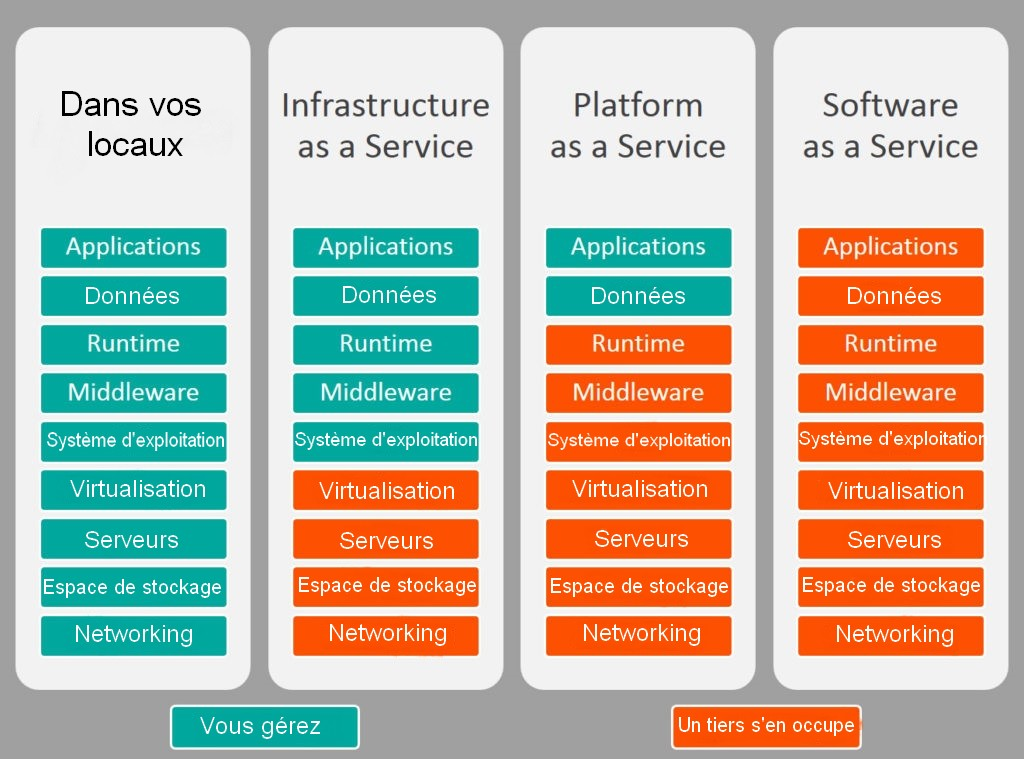
\includegraphics[scale=.4]{img/modeles.jpg}
        \caption{Services gérés par le fournisseur ou par le client en
        fonction du modèle \\ Source : \url{https://architecture-cloud.fr}}
      \end{figure}
      \label{fig:modeles}
  \end{spacing}
\end{document}
